\documentclass[10pt,aspectratio=169]{beamer}

\usepackage[T1]{fontenc}
\usepackage[utf8]{inputenc}
\usepackage[french]{babel}
\usepackage{lmodern}
\usepackage{booktabs}
\usepackage{array}
\usepackage{graphicx}
\usepackage{adjustbox}
\usepackage{multicol}
\usepackage{xcolor}
\usepackage{hyperref}

\graphicspath{{images/}}

\usetheme{Madrid}
\usecolortheme{seagull}

\definecolor{seerGreen}{HTML}{2E7D32}
\definecolor{seerRed}{HTML}{C62828}
\definecolor{seerOrange}{HTML}{E65100}
\definecolor{seerBlue}{HTML}{1E4E8C}

\setbeamercolor{palette primary}{bg=seerBlue, fg=white}
\setbeamercolor{palette secondary}{bg=seerGreen, fg=white}
\setbeamercolor{palette tertiary}{bg=seerOrange, fg=white}
\setbeamercolor{structure}{fg=seerBlue}
\setbeamercolor{title}{fg=seerBlue}
\setbeamercolor{frametitle}{fg=white,bg=seerBlue}

\title[Application RLM]{Application de la régression logistique multinomiale}
\subtitle{Données SEER : cause de décès chez les patients cancéreux}
\author{DOSSOU YOVO Thérèse \and GLODJO Jolémon}
\date{11 avril 2026}

\AtBeginSection[]
{
  \begin{frame}{Plan de la section}
    \tableofcontents[currentsection]
  \end{frame}
}

\begin{document}

\begin{frame}
  \titlepage
\end{frame}

\begin{frame}{Fil conducteur de l’application}
\begin{enumerate}
  \item Présentation des données et des variables.
  \item Analyse exploratoire détaillée.
  \item Vérification des conditions d’application.
  \item Ajustement du modèle multinomial.
  \item Interprétation des coefficients et validation.
  \item Conclusion et discussion.
\end{enumerate}
\vspace{0.5em}
\textbf{Idée directrice :} expliquer la cause de décès par des facteurs cliniques et sociodémographiques, en prenant \textit{Alive} comme catégorie de référence.
\end{frame}

\begin{frame}{Présentation des données}
\begin{columns}[T,onlytextwidth]
  \column{0.58\textwidth}
  \begin{itemize}
    \item Base SEER nettoyée et recodée pour une réponse multinomiale à trois modalités.
    \item Taille finale : 3000 observations après suppression des valeurs manquantes sur les variables du modèle.
    \item Variable dépendante : \textit{Csdc} = Alive / Dead (attributable to this cancer dx) / Dead of other cause.
    \item Référence choisie : \textit{Alive}.
    \item Variables explicatives : âge, sexe, race, site primaire, grade, stade, chimiothérapie.
  \end{itemize}
  \column{0.42\textwidth}
  \begin{block}{Codage retenu}
  \small
  \begin{tabular}{@{}ll@{}}
  \toprule
  \textbf{Type} & \textbf{Variables} \\
  \midrule
  Nominales & Sex, Race, Primarysite, Chemotherapy, Status \\
  Ordinales & Grade, Stage \\
  Réponse & Csdc \\
  \bottomrule
  \end{tabular}
  \end{block}
\end{columns}
\end{frame}

\begin{frame}{Aperçu des premières observations}
\begin{figure}
  \centering
  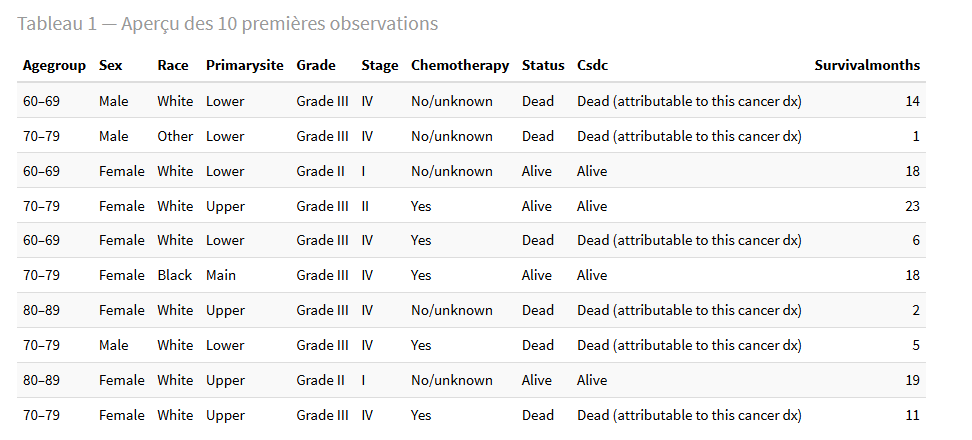
\includegraphics[width=0.98\linewidth]{Apercu.png}
\end{figure}
\vspace{-0.8em}
\footnotesize Le tableau sert à vérifier la structure des variables, les modalités et le bon encodage avant l’analyse.
\end{frame}

\begin{frame}{Distribution de la variable réponse}
\begin{figure}
  \centering
  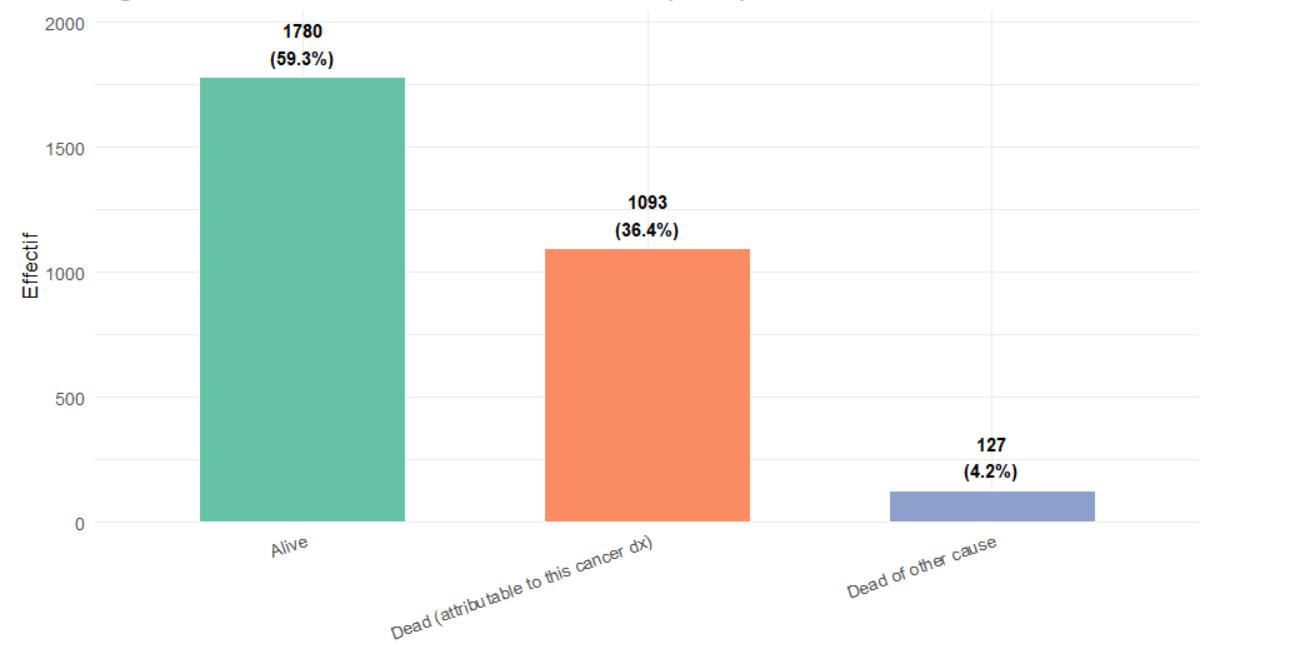
\includegraphics[width=0.96\linewidth]{distribution_csdc.png}
\end{figure}
\vspace{-0.5em}
\begin{itemize}
  \item \textit{Alive} domine l’échantillon : 1780 cas, soit 59,3\%.
  \item \textit{Dead (attributable to this cancer dx)} : 1093 cas, soit 36,4\%.
  \item \textit{Dead of other cause} : 127 cas, soit 4,2\%.
\end{itemize}
\end{frame}

\begin{frame}{Survie selon la cause de décès}
\begin{columns}[T,onlytextwidth]
  \column{0.56\textwidth}
  \begin{figure}
    \centering
    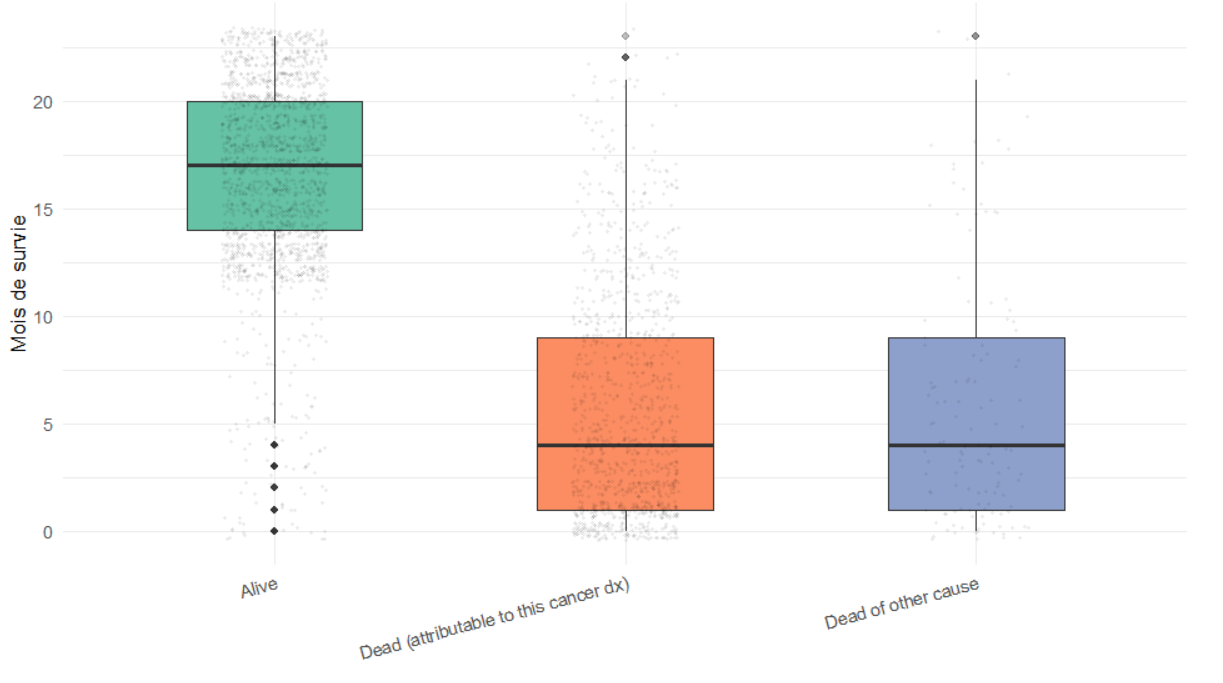
\includegraphics[width=\linewidth]{boxplotdiscsdc.png}
  \end{figure}
  \column{0.44\textwidth}
  \begin{figure}
    \centering
    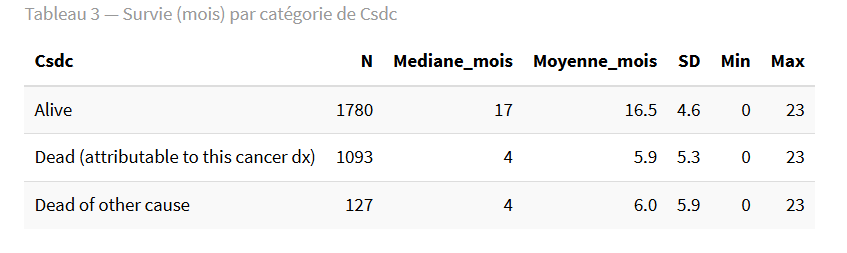
\includegraphics[width=\linewidth]{survie_categories.png}
  \end{figure}
\end{columns}
\vspace{-0.6em}
\begin{itemize}
  \item Les patients vivants ont une médiane de survie nettement plus élevée.
  \item Les décès attribuables au cancer présentent une survie médiane très courte.
  \item Les décès d’autre cause sont plus dispersés, ce qui suggère une hétérogénéité clinique.
\end{itemize}
\end{frame}

\begin{frame}{Association bivariée entre Csdc et les covariables}
\begin{columns}[T,onlytextwidth]
  \column{0.52\textwidth}
  \begin{figure}
    \centering
    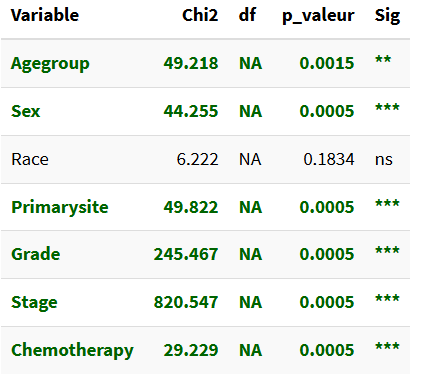
\includegraphics[width=\linewidth]{assoki2.png}
  \end{figure}
  \column{0.48\textwidth}
  \begin{block}{Lecture du test de Khi-deux}
  \small
  Les associations sont fortes pour :
  \begin{itemize}
    \item Agegroup
    \item Sex
    \item Primarysite
    \item Grade
    \item Stage
    \item Chemotherapy
  \end{itemize}
  Race ressort comme la seule variable non significative dans ce tableau bivarié.
  \end{block}
\end{columns}
\end{frame}

\begin{frame}{Conditions d’application}
\begin{columns}[T,onlytextwidth]
  \column{0.5\textwidth}
  \begin{block}{Diagnostics vérifiés dans le Rmd}
  \begin{itemize}
    \item Multicolinéarité : VIF/GVIF contrôlé, sans alerte majeure.
    \item Dispersion : ratio de Pearson proche de 1.
    \item Séparation parfaite : absence de problème détecté.
    \item IIA : test réservé après l’ajustement du modèle.
  \end{itemize}
  \end{block}
  \column{0.5\textwidth}
  \begin{block}{Conséquence méthodologique}
  Le modèle multinomial standard est justifié, car les hypothèses de base ne sont pas violées de manière visible.
  \end{block}
\end{columns}
\end{frame}

\begin{frame}{Qualité d’ajustement du modèle}
\begin{figure}
  \centering
  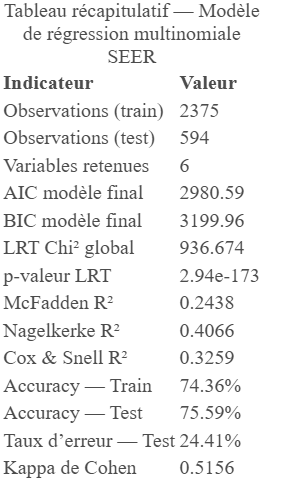
\includegraphics[width=0.72\linewidth]{ajustement.png}
\end{figure}
\vspace{-0.5em}
\begin{center}
\small
\begin{tabular}{@{}l r@{}}
\toprule
\textbf{Métrique} & \textbf{Valeur} \\
\midrule
Log-vraisemblance (modèle complet) & -1825.1700 \\
Log-vraisemblance (modèle nul) & -2434.3400 \\
AIC & 3738.3500 \\
BIC & 4002.6300 \\
McFadden $R^2$ & 0.2502 \\
Cox \& Snell $R^2$ & 0.3338 \\
Nagelkerke $R^2$ & 0.4159 \\
\bottomrule
\end{tabular}
\end{center}
\end{frame}

\begin{frame}{Coefficients, OR et significativité}
\begin{columns}[T,onlytextwidth]
  \column{0.5\textwidth}
  \begin{figure}
    \centering
    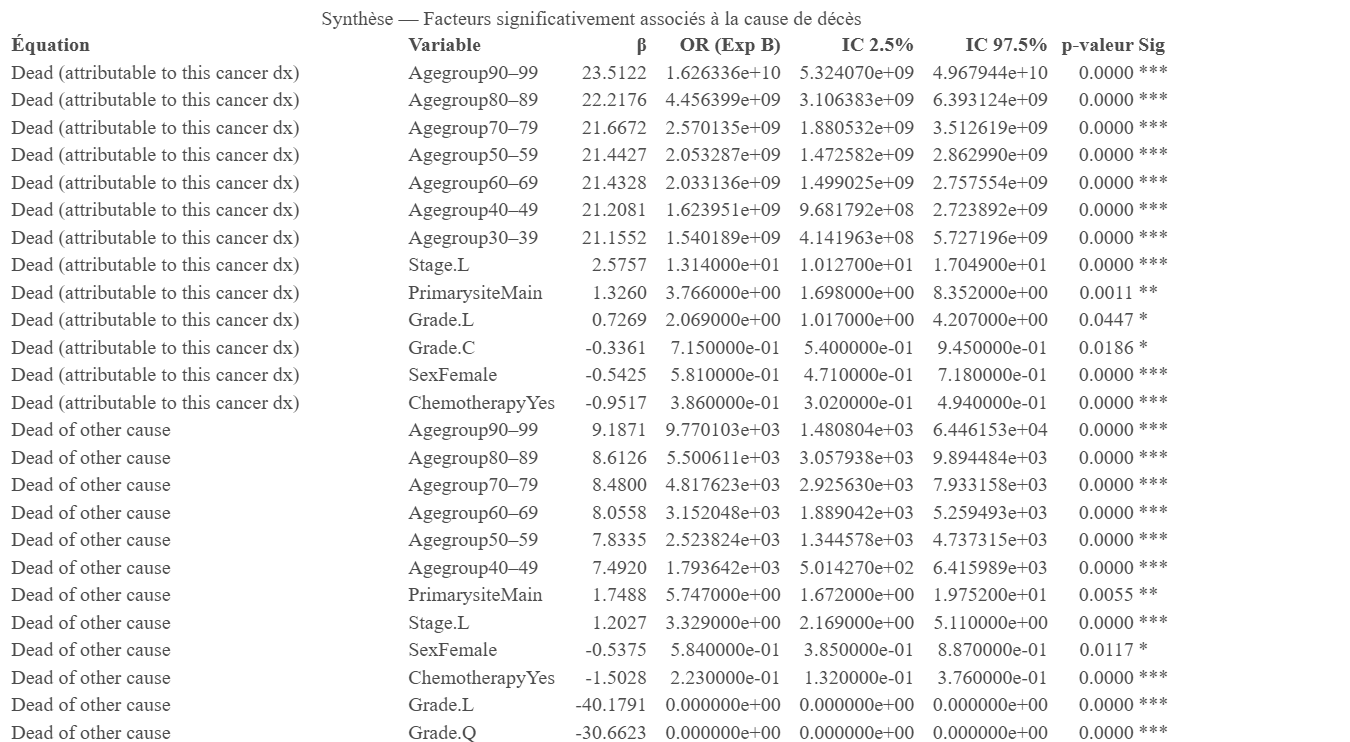
\includegraphics[width=\linewidth]{OR1.png}
  \end{figure}
  \column{0.5\textwidth}
  \begin{figure}
    \centering
    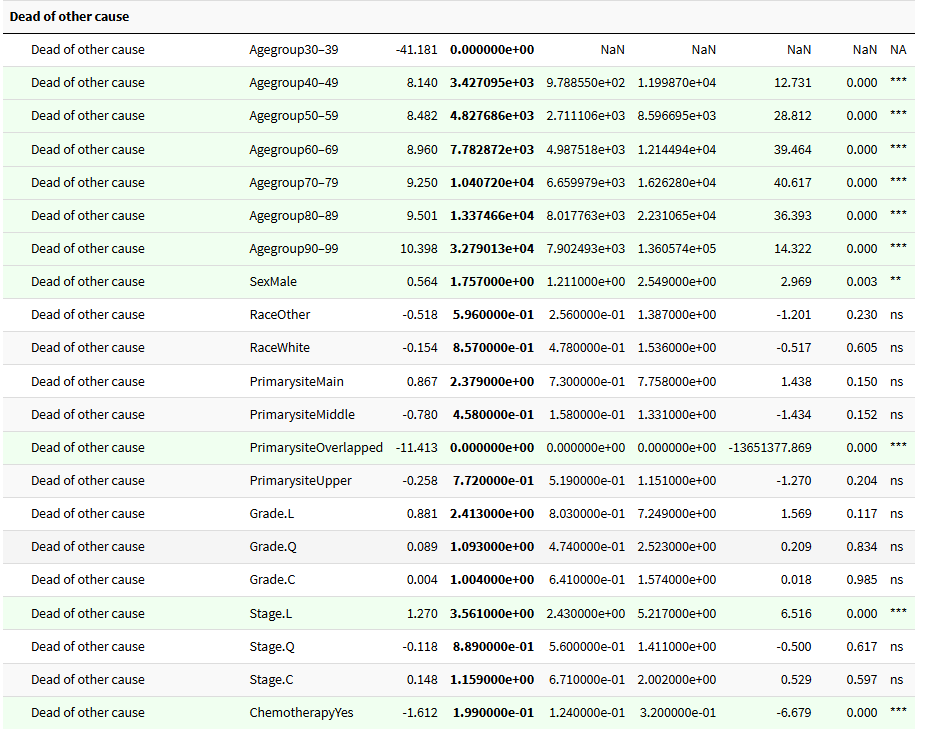
\includegraphics[width=\linewidth]{OR1suite.png}
  \end{figure}
\end{columns}
\vspace{-0.5em}
\begin{itemize}
  \item Les OR très élevés sur les classes d’âge traduisent un effet de gradient prononcé.
  \item Le stade tumoral et le grade ressortent comme déterminants majeurs.
  \item La chimiothérapie doit être interprétée avec prudence à cause du biais d’indication.
\end{itemize}
\end{frame}

\begin{frame}{Matrice de confusion et validation prédictive}
\begin{columns}[T,onlytextwidth]
  \column{0.56\textwidth}
  \begin{figure}
    \centering
    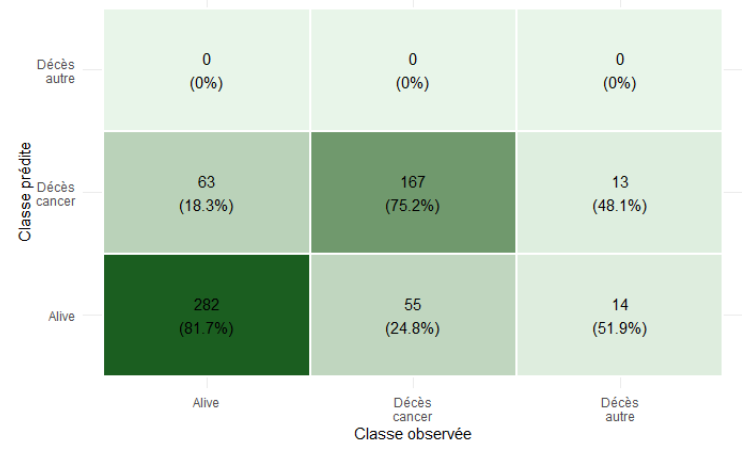
\includegraphics[width=\linewidth]{matriceconfusion.png}
  \end{figure}
  \column{0.44\textwidth}
  \begin{block}{Lecture rapide}
  \small
  \begin{itemize}
    \item La diagonale concentre l’essentiel des bonnes classifications.
    \item L’accuracy globale est d’environ 74,5\%.
    \item Le modèle discrimine correctement les classes majoritaires, avec une précision plus faible pour la classe rare.
  \end{itemize}
  \end{block}
\end{columns}
\end{frame}

\begin{frame}{Probabilités prédites moyennes}
\begin{columns}[T,onlytextwidth]
  \column{0.5\textwidth}
  \begin{figure}
    \centering
    
\includegraphics[width=\linewidth]{result.png}
  \end{figure}
  \column{0.5\textwidth}
  \begin{block}{Valeurs observées}
  \small
  \begin{tabular}{@{}lr@{}}
  \toprule
  \textbf{Catégorie} & \textbf{Probabilité moyenne} \\
  \midrule
  Alive & 0.5933 \\
  Dead (attributable to this cancer dx) & 0.3643 \\
  Dead of other cause & 0.0423 \\
  \bottomrule
  \end{tabular}
  \end{block}
  \vspace{0.8em}
  \begin{itemize}
    \item Ces probabilités résument l’équilibre global du modèle.
    \item La classe \textit{Alive} reste la plus probable en moyenne.
  \end{itemize}
\end{columns}
\end{frame}

\begin{frame}{Synthèse des résultats statistiques}
\small
\begin{table}
\centering
\begin{tabular}{@{}lccc@{}}
\toprule
\textbf{Variable} & \textbf{$\chi^2$} & \textbf{p-value} & \textbf{Conclusion} \\
\midrule
Agegroup & 49.218 & 0.0005 & Significative \\
Sex & 44.255 & 0.0005 & Significative \\
Race & 6.222 & 0.1779 & Non significative \\
Primarysite & 49.822 & 0.0005 & Significative \\
Grade & 245.467 & 0.0005 & Significative \\
Stage & 820.547 & 0.0005 & Significative \\
Chemotherapy & 29.229 & 0.0005 & Significative \\
\bottomrule
\end{tabular}
\end{table}
\vspace{0.5em}
\begin{itemize}
  \item Le stade est le prédicteur le plus fortement associé à la cause de décès.
  \item Le grade et l’âge apportent aussi une information importante.
  \item La race ne ressort pas comme déterminante dans l’analyse bivariée.
\end{itemize}
\end{frame}

\begin{frame}{Discussion}
\begin{itemize}
  \item Le stade tumoral domine l’explication de la mortalité spécifique, ce qui est cohérent avec la littérature oncologique.
  \item Le grade élevé traduit une agressivité biologique accrue et s’accompagne d’un risque plus élevé de décès par cancer.
  \item L’effet apparent de la chimiothérapie doit être lu comme un effet de sélection clinique, non comme une causalité directe.
  \item Les variables sociodémographiques gardent une utilité explicative, mais leur interprétation doit rester prudente.
\end{itemize}
\vspace{0.5em}
\begin{block}{Limite importante}
La régression multinomiale décrit des associations et ne remplace pas une analyse causale ou un modèle de survie.
\end{block}
\end{frame}

\begin{frame}{Conclusion}
\begin{itemize}
  \item La démarche suit une logique complète : préparation, exploration, contrôle des hypothèses, estimation et validation.
  \item Le modèle multinomial est globalement pertinent pour expliquer les trois issues de décès.
  \item Les facteurs les plus structurants sont le stade, le grade et l’âge.
  \item La performance prédictive est correcte, mais l’interprétation clinique reste prioritaire sur la seule accuracy.
\end{itemize}
\vspace{0.7em}
\centering
\textbf{Message final :} la méthode est cohérente et robuste pour une lecture explicative des causes de décès, à condition de garder en tête ses limites d’inférence causale.
\end{frame}

\end{document}